\chapter{Estado del arte}
\label{ch:chap02}

\section{Modelos de iluminación}
\label{sec:dibujado}

El proceso de dibujado de gráficos por computadora comprende la generación automática de imágenes a partir de una escena virtual.
Definida por su geometría (la disposición espacial de los objetos de una escena), la posición de la cámara y características ambientales 
como las luces y materiales que componen las superficies.

Cuando se dibujan objetos tridimencionales, es necesario establecer un modelo de interacción entre las superficies y
la luz. En este sentido, existen dos modelos de iluminación: local y global.

\begin{minipage}[h]{0.8\linewidth}
    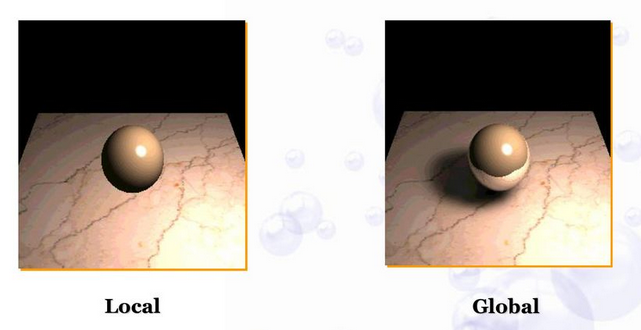
\includegraphics[width=\linewidth]{assets/local_vs_global}
    \captionof{figure}{Dibujado utilizando iluminación local y global}
    \label{local-vs-global-img}
\end{minipage}

\section{Iluminación local}
\label{sec:ilumlocal}
Los modelos de iluminación local como\cite{Phong} tienen en cuenta las propiedades físicas de los materiales
y las superficies de cada uno de los objetos de la escena de forma individual. Es decir, al dibujar uno de los
objetos no se toman en cuenta las posibles interacciones de los haces de luz con los objetos restantes.

\section{Iluminación Global}
\label{sec:ilumglobal}

El término iluminación global refiere a una modelo de
computación gráfica que simula completament interacciones de la luz con todos los objetos que se encuentran 
en la escena. Es decir, en contraposición a la iluminación local, se consideran los fenómenos de
reflexión y refracción de la luz.

Por lo cual, el objetivo final de la computación obtener un valor para la radiancia de cada punto del espacio. Desde un punto de vista
matemático, todos los modelos de iluminación global existentes resuelven la ecuación de \textit{rendering} de Kajiya.

\begin{equation}
    I(x,x') = g(x,x') \bigg[\epsilon(x,x') + \int_{S} \rho(x,x',x'')I(x',x'') \delta x''\bigg]
\end{equation}
donde:
\begin{itemize}
    \item $I(x,x')$ describe energía de radiación desde el punto $x'$ a $x$
    \item $g(x,x')$ es un término geométrico, toma el valor de $0$ si existe oculsión entre $x'$ y $x$ en otro caso su valor es $\dfrac{1}{r^{2}}$ donde $r$ es la distancia entre $x'$ y $x$
    \item $\epsilon(x,x')$ mide la energía emitida por la superficie en el punto $x'$ a $x$
    \item $\int_{S} \rho(x,x',x'')I(x',x'') \delta x''$ está compuesta por dos términos:
        \begin{itemize}
            \item $\rho(x,x',x'')$ es el término de dispersión de la luz que llega desde $x''$ a $x$ desde el punto $x'$
            \item $I(x',x'')$ describe energía de radiación desde el punto $x''$ a $x'$
        \end{itemize}
    por lo que este término refiere a la intensidad percibida desde $x$ considerando todos las reflexiones de
    luz posibles para el espacio $S$.
\end{itemize}

Su significado se puede resumir de la siguiente manera: para calcular la radiancia observada en el punto $x$ desde $x'$  es necesario agregar
la intensidad de luz emitida desde $x'$ con las intensidades de todos los puntos de la escena que se reflejan a $x$ desde $x'$.

\section{Radiosidad}
\label{sec:radiosidad}

\subsection{Radiosiodad}

\section{Rasterización}
\label{sec:rasterizacion}

\subsection{OpenGL}
\label{sec:opengl}

\section{Raytracing}
\label{sec:raytracing}

\subsection{Embree}
\label{sec:embree}
